\chapter{背景与相关工作定位}

可编辑音频效果控制的难点来自一个非对称关系：用户通常用自然语言描述感知目标，例如 warm、tight、clean、heavy 或 ambient；插件实际执行的却是多模块参数向量。该向量包括压缩器、失真、过载、延迟、混响、合唱、镶边、均衡和相位等模块的开关状态与数值参数。自然语言、参考音频和参数向量之间没有一一对应关系，因此直接让语言模型生成参数容易出现数值漂移，直接使用通用音频嵌入也未必能对齐插件参数空间。

检索式方法为该问题提供了一个可审计中间层。系统不需要从零生成所有参数，而是在已有知识库中寻找相似预设，并输出该预设的真实参数。检索结果的优点是可执行、可检查、可复用；缺点是性能受数据库覆盖、切分质量和相似度定义限制。Audio-Agent 当前实验正是在这个折中点上展开：它评估不同检索表示是否能够更稳定地找到参数空间上接近 ground truth 的候选。

在当前代码库中，实验证据与产品链路应当分开理解。产品链路包含 DeepSeek 风格解析、MusicGen 音频生成、JUCE 插件参数导入与离线渲染；实验链路则主要围绕外部 1267 条 benchmark 数据、缓存向量和参数 JSON 展开。本文的主结论来自实验链路，尚未覆盖完整插件输出音频质量。这个区分很重要，因为参数空间评价能够支持 retrieval prior 的有效性，却不能自动证明端到端听感最优。

现有论文材料已经对主张进行了收敛。提交面文稿将主贡献限定为 retrieval-grounded editable preset control，并在本轮根据用户已 double check 的 P0 E3 结果，把 real-audio degradation robustness 从“待补实验”升级为“当前退化集合下的 fusion 证据”。本报告仍将证据层分为 source claim、repo-observed fact、已确认正式实验数据、design intent 和 report synthesis。凡是只存在于计划或脚本中的内容，仍不能被写成已经验证的事实；P0 E2/E3 则按已确认真实、完整、正确的正式实验数据处理。

\begin{figure}[H]
	\centering
	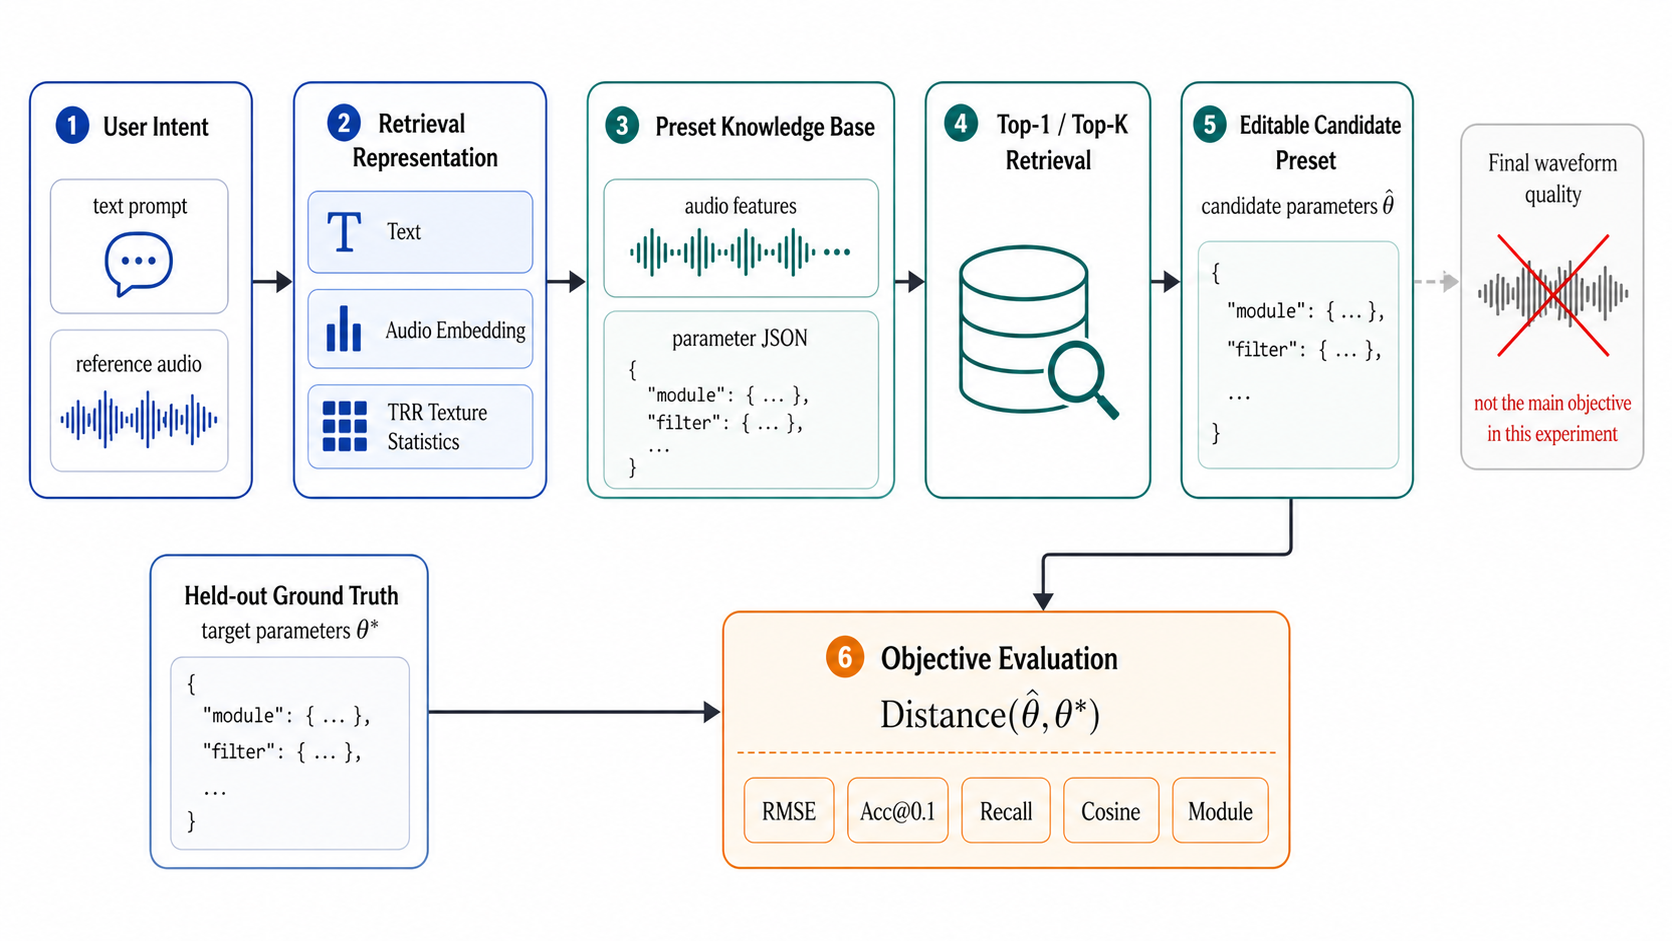
\includegraphics[width=\textwidth]{figures/retrieval-control-problem.png}
	\caption{本文关注的检索式可编辑参数控制问题。主实验评价检索候选与 ground-truth 参数之间的距离，不直接评价最终波形质量。}
	\label{fig:retrieval-control-problem}
\end{figure}

图~\ref{fig:retrieval-control-problem} 展示了本文的研究边界。TRR 的角色是改善检索表示，使系统更可能从知识库中取回参数邻域正确的候选；它不是完整的 DAW 代理、不是端到端主观优化器，也不是替代所有音频表示的通用模型。
